%
%
%

%
% Use the standard article template.
%
\documentclass{article}

% The geometry package allows for easy page formatting.
\usepackage{geometry}
\geometry{letterpaper}

% Load up special logo commands.
\usepackage{doc}

% Package for formatting URLs.
\usepackage{url}

% Packages and definitions for graphics files.
\usepackage{graphicx}
\usepackage{epstopdf}
\DeclareGraphicsRule{.tif}{png}{.png}{`convert #1 `dirname #1`/`basename #1 .tif`.png}

%
% Set the title, author, and date.
%
\title{Predicting Credit Card Defaults \\ EECS 433 Final Project}
\author{Jason Brown\\
 M.S. Computer Science \\ Northwestern University \\
  \texttt{jasonbrown2016@u.northwestern.edu}}
\date{March 2016}

%
% The document proper.
%
\begin{document}

% Add the title section.
\maketitle

% Add an abstract.
\abstract{
This paper uses multiple machine learning algorithms, such as K-nearest neighbor, Logistic regression, Discriminant analysis, Na�ve Bayesian, and Classification tree, to predict credit card defaults from a sample of $n= 30,000$. It uses baseline techniques and seeks to show how selected improvements to the algorithms can be made that result in slightly better model accuracy, as judged by the Receiver Operating Characteristic \textit{area under curve} metric. The paper concludes with a discussion of the strengths and weaknesses of the algorithms, and the reason why the Na�ve Bayesian approach yielded the best model performance.
}

% Add various lists on new pages.
\pagebreak
\tableofcontents

\pagebreak
\listoffigures

\pagebreak
\listoftables

% Start the paper on a new page.
\pagebreak

%
% Body text.
%
\section{Introduction \& Motivation}
\label{introduction}

You will almost certainly start with an introductory description of the topic that you investigated in your assignment.  Discuss any goals, motivation, or examples of the subject; the key is to provide the reader with any information that is necessary to understand why your topic was worth investigating.  This descriptive section should also allow the reader to understand the subsequent detail sections on the subject.

\section{Problem Description}

\subsection{Description of the Data}

The data is comprised of 23 explanatory variables ($X1$-$X23$) and one response variable ($Y$). $Y$ denotes whether the borrower defaulted on credit card debt repayment, with $Y=1$ denoting default. In the sample size of $n= 30,000$, only $6,636$ ($22\%$) defaulted. 

\begin{table}
\centering
\begin{tabular}{|c|c|c|}\hline
Label & Attribute & Notes \\\hline\hline
X1 & Credit Given &  NT Dollar currency\\
X2 & Gender & 1= male, 2 = female \\
X3 & Education & 1 = grad. school; 2 = university; 3 = high school \\
X4 & Marital Status & 1 = married; 2 = single\\
X5 & Age & years \\
X6 & Repayment Status- Sept & -1 = pay duly; 1 = 1mo payment delay; $\dots$ \\
X7 & Repayment Status- Aug & $\dots$ 9 = 9mo payment delay or greater \\
X8 & Repayment Status- July & -\\
X9 & Repayment Status- June & -\\
X10 & Repayment Status- May & -\\
X11 & Repayment Status- April &- \\
X12 & Bill Statement- Sept & NT Dollary currency \\
X13 & Bill Statement- Aug & -\\
X14 & Bill Statement- July & -\\
X15 & Bill Statement- June &-\\
X16 & Bill Statement- May & -\\
X17 & Bill Statement- April &-\\
X18 & Bill Payment- Sept & NT Dollary currency \\
X19 & Bill Payment- Aug & -\\
X20 & Bill Payment- July & -\\
X21 & Bill Payment- June &-\\
X22 & Bill Payment- May & -\\
X23 & Bill Payment- April &-\\\hline
\end{tabular}

\caption{Explanatory Variables}
\label{table-Variables}
\end{table}

\subsection{Measuring Model Accuracy}

When the explanatory variable is skewed towards one binary value, as is the case here, measuring the accuracy of a model via its error rate is insufficient. Consider a naive model that estimated $\hat{y} = 1$ regardless of the values of the explanatory variables. Despite this being a naive and model that added little value, it would have a decent error rate: Consider $n=100$, this model would then have $\approx 22$ 
misclassifications, resulting in an error rate of 22\%. That's not half-bad!

While error rate is often a good measure of model accuracy, it is clearly insufficient here. A better measure of model accuracy involves using a lift curve. Let's consider a sample of $n=100$ with probility of $y$ of 22\%. Three lines comprise a lift curve: i) the prior probability line which represents a guess; this line would start at (0,0), and extend to (100,22) with slope 11/50. ii) The hypothetical best-model, which would start at (0,0), extend to (22,22) with slope 1, and then extend to (100,22) with slope 0. This curve represents 100\% accuracy, or the ability to pick out which of the 100 samples have response variable equal to one. Lastly, iii) represents the model. This would hopefully be able to ascertain which of the $n=100$ are likely to yield $y=1$, and pick those first. The accuracy measure uses the ratio between the lines ((iii) \& (i)) divided by ((ii) \& (i)). A good model will be closer to the hypothetical best line than to the guess line, so it will have a ratio approaching 1.

Receiver operating characteristic (ROC) \textit{area under curve} is also a good measure of model accuracy. An ROC curve measures the discriminability of a model. It plots the true positive rate as a function of the false positive rate. Each point represents a specificity pair; the curve has higher slope initially because in a gaussian distribution, there are values on both sides of the bell curve that are easy to classify. The slope approaches 0 as the curve gets closer to 100\% true sensitivity rate, as there will always be instances that are very tough to classify, for which the model would yield false positives before it found a true positive. The area under the curve represents the quality of the model, where 1 is the hypothetical best model. The ROC curves for the models utilized in this paper are presented in Figure 1. The best performing model had an area under curve ratio of 75\%.

\begin{figure}
\centering
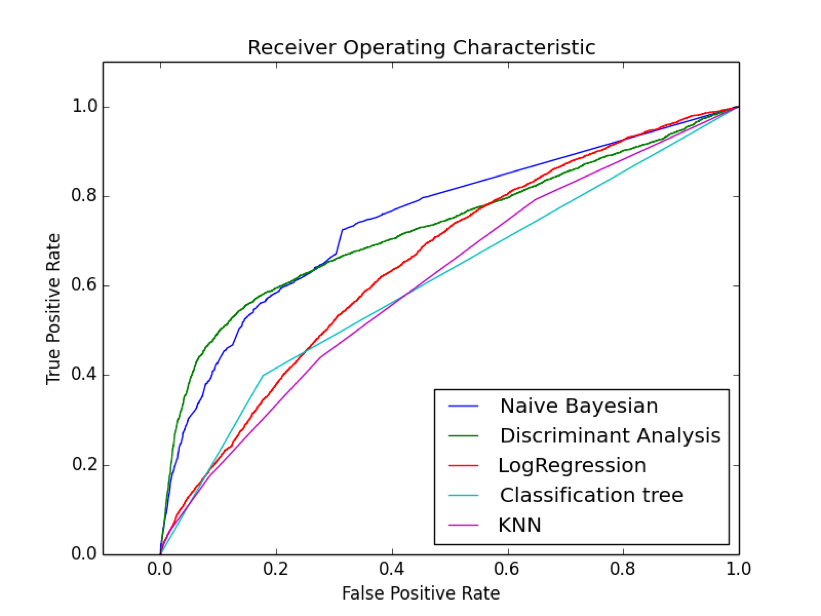
\includegraphics[width=5in]{images/ROC.png} 

\caption{Receiver Operating Characteristic}
\label{ROC area under curve}
\end{figure}

\subsection{Not all Misclassifications are Equal}

The section above treats a false positive and a false negative equal in the eyes of the model accuracy rates. However, this is not the case in actuality; one misclassification may be considerably more costly to the end user of the model than another type of misclassification. Consider a radiologist screening for cancer; a false positive would scare a patient, but a false negative is far worse - it could lead to the cancer going untreated. Similarly, consider a bank using the credit card data to decide whether to issue credit to a customer. A false positive would represent major loss from default on debt (Figure 2 - upper right quadrant), whereas a false negative would represent a minor loss of revenue from the client under consideration (Figure 2 - lower left quadrant).

\begin{figure}
\centering
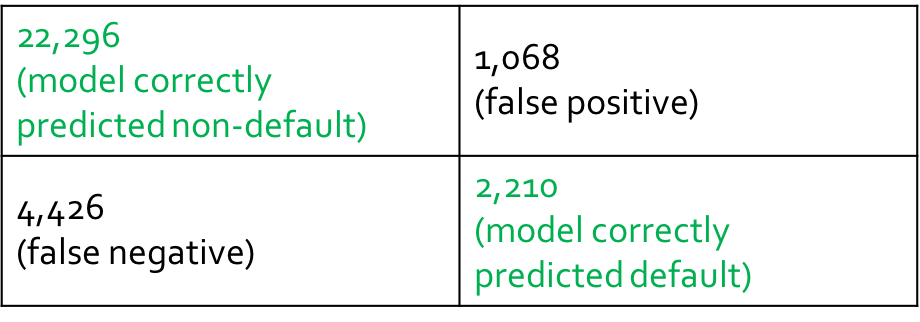
\includegraphics[width=3in]{images/confusion_matrix.png} 

\caption{Confusion Matrix - KNN}
\label{Confusion Matrix - KNN}
\end{figure}

\section{Baseline Methods}

This section will the discuss the baseline methods used to predict credit card defaults.

\subsection{Classification Tree}

Splitting the data set of $n=30,000$ into $n=15,000$ for training and $n=15,000$ for testing; a decision tree classifier was trained with the training set. A decision tree starts at the root of the tree; each attribute is considered for its \textit{information gain}; whichever attribute best splits the yes / no classifications correctly is chosen as the root of the subtree. Here, \textit{best} is measured based on relative entropic purity of potential children nodes. Entropy 

\\

A Classification tree model represents a \textit{greedy} algorithm since it is based on making a series of locally-best decisions until a base case is reached; in a decision tree, the base case is correct classification; however, pruning can be used to prevent \textit{overfitting} and a model that generalizes better.





\begin{figure}
\centering
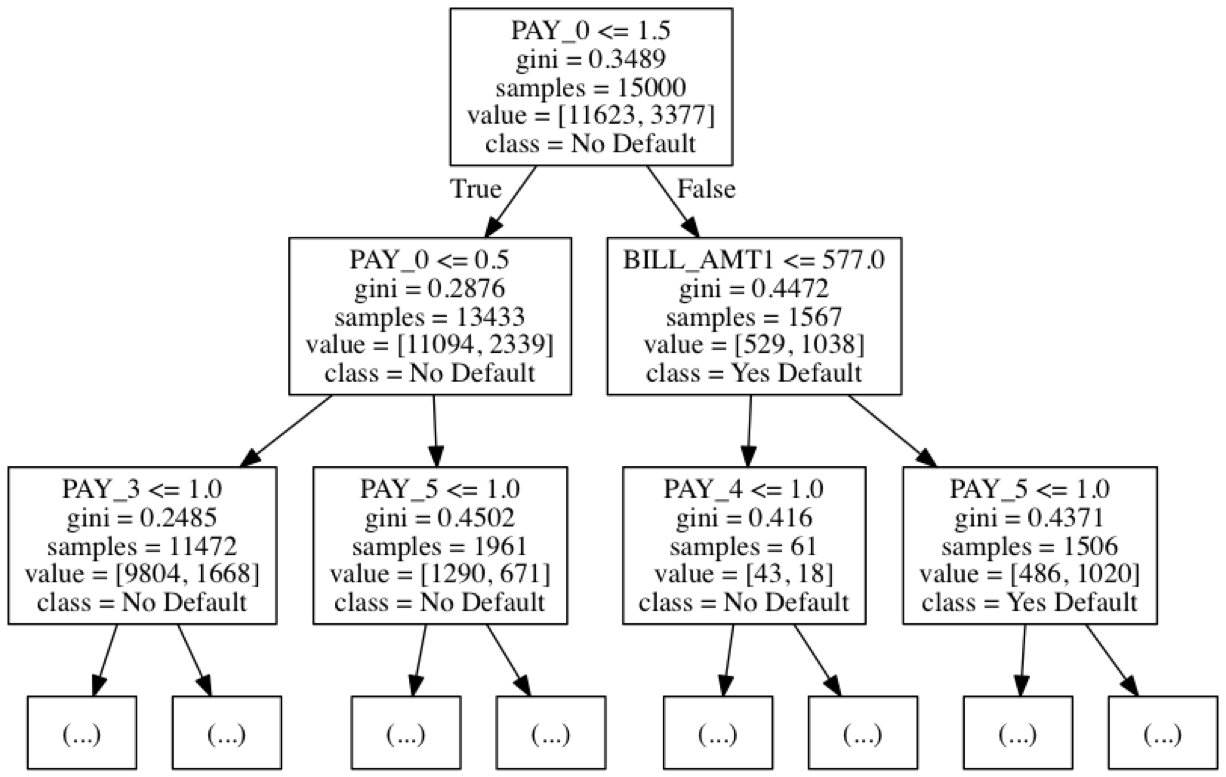
\includegraphics[width=5in]{images/decision_tree_baseline.png} 

\caption{Decision Tree - prior to feature selection}
\label{Decision Tree - prior to feature selection}
\end{figure}

\subsection{K-Nearest Neighbor}

xyz

\subsection{Logistic Regression}

xyz

\subsection{Discriminant Analysis}

xyz

\subsection{Naive Bayesian}

xyz

\section{Improvements}

\subsection{Feature Selection}

xyz

\subsection{10-Fold Cross Validation}

xyz

\subsection{Principal Component Analysis}

xyz

\section{Conclusion}

Wrap up your paper with an ``executive summary'' of the paper itself, reiterating its subject and its major points.  If you want examples, just look at the conclusions from the literature.

\section{Course Feedback}

Professor Wu is clearly an accomplished researcher and this course is very advanced and well taught; I particularly liked the demos on the chalkboard. Students would have benefited from mandatory assignments from the book to solidify the materials taught in lecture; applying what we've learned helps reenforce learning new material. Similarly, weekly office hours, a teaching assistant, and piazza, would have led to discussions that would have benefited all students and furthered learning. A really solid background in linear algebra would have helped me more-easily understand the fast-moving lectures. I'm pleased I took the course, and it has opened doors for future statistical pattern recognition learning down-the-road.

\section{Latex Features}

\subsection{Tables and Figures}

\LaTeX\ has full support for tables and figures.  Table~\ref{table-sample} shows a sample table and Figure~\ref{figure-sample} shows a sample figure.  Note the built-in support for captions and the automated numbering functionality.  Lists of tables and figures can also be automatically generated, as seen at the beginning of this document.

\begin{table}
\centering
\begin{tabular}{|c|c|c|}\hline
Column 1 & Column 2 & Column 3 \\\hline\hline
a & b & c \\
d & e & f \\
g & h & i \\\hline
\end{tabular}

\caption{A sample table}
\label{table-sample}
\end{table}



One very important thing to remember about how \LaTeX\ handles tables and figures by default: you don't have to worry about where they go exactly.  The general rule is that you insert them in the source after your first reference to them, and \LaTeX\ determines their final position.  It also makes decisions on how much page space to devote to them.  This all follows \LaTeX's overall theme of focusing on the content of your paper, and not its format.

Just so you can see a second table, Table~\ref{table-sample2} is provided.

\begin{table}
\centering
\begin{tabular}{|c|c|c|}\hline
Column 1 & Column 2 & Column 3 \\\hline\hline
a & b & c \\
d & e & f \\
g & h & i \\\hline
\end{tabular}

\caption{Another sample table}
\label{table-sample2}
\end{table}

\section{Latex features}

Perhaps the most important functionality to learn for the paper is \LaTeX\ bibliography support.  Citations and references are handled automatically by \LaTeX\ through its companion program, \BibTeX.  All you have to do is provide a bibliography file that provides the reference information and internal keys (very much like variable names) that you use in your document.\footnote{And always remember to run \LaTeX\ \emph{at least twice} after running \BibTeX.}

\BibTeX\ supports virtually all kinds of references, including books \cite{dui,sgg,iokit,palmos}, parts of books \cite{userModeLinux}, articles \cite{nielsen:dui-review,heer-shneiderman,stackableThreads,xpkernel}, and conference proceedings \cite{ux-3d,iring,contextFileSearch,osHaskell,hibernator}, to name a few.  If not already included in your \LaTeX\ distribution, download and install the \texttt{url} package to support formatting of URLs; you can usually mention these in the \emph{note} or \emph{howpublished} fields of your \BibTeX\ file.

Like Section~\ref{introduction}, a background, preliminary, and related work section is also almost certainly needed for your paper.  In this section, describe any history, work, or projects that serve as direct contributors to the subject of your research paper.  Look at other papers in the literature to see how they organized, presented, and discussed prior work.

The Shneiderman/Plaisant text \cite{dui} provide some pointers to seminal or key works; because they made it into the textbook they aren't necessarily ``bleeding edge,'' but they likely provide the foundation for your chosen subject matter.

\section{Another Section}

We're adding another section just so you can see how that looks.  Plus there are a few more \LaTeX\ features to illustrate.

\subsection{Bulleted and Numbered Lists}

\LaTeX\ is very good at providing clean lists.  Examples are shown below.

\begin{itemize}
\item Bulleted items come out properly indented and spaced, every time.

\begin{itemize}
\item Sub-bullets are a virtual no-brainer: just nest another \verb!itemize! block.
\item Note how the bullet character automatically changes too.
\end{itemize}

\item Just keep on adding \verb!\item!s\ldots

\item \ldots until you're done.
\end{itemize}

Numbered lists are almost identical, except that you specify \verb!enumerate! instead of \verb!itemize!.  List items are specified in exactly the same way (thus making it easy to change list types).

\begin{enumerate}
\item A list item
\item Another list item
\item A list item with multiple nested lists

\begin{itemize}
\item Nested lists can be of mixed types.
\item That's a lot of power and flexibility for the price of learning a handful of directives.

\begin{enumerate}
\item Like nested bullet lists, nested numbered lists also ``intelligently'' change their numbering schemes.
\item Meanwhile, all \emph{you} have to write is \verb!\item!.  \LaTeX\ does the rest.
\end{enumerate}
\end{itemize}

\item Back to your regularly scheduled list item

\end{enumerate}

\subsection{Subsection with Another Figure}

We may as well include a second figure also, shown in Figure~\ref{figure-sample2}.  The same image file is used, but note how it can be resized.  Again, observe how the positions of the tables and figures do not necessarily match their positions in the source file, reiterating the aforementioned \LaTeX\ functionality for deciding where these items go in the final document.  You provide an approximate location, and \LaTeX\ does the rest.

\begin{figure}
\centering
%\includegraphics[width=1in]{space.jpg} 

\caption{Another sample figure}
\label{figure-sample2}
\end{figure}

% Generate the bibliography.
\bibliography{latex-sample}
\bibliographystyle{unsrt}

\end{document}
